\section{Resoconto delle attività di verifica}
\label{resoconto}
\subsection{Periodo di analisi e consolidamento dei requisiti}
Durante questi periodi, i documenti redatti da presentare in ingresso alla \textbf{Revisione dei Requisiti} sono stati verificati dai \textit{Verificatori} secondo i criteri per l'analisi statica definiti nelle \NdPv{1.0.0}, seguendo le metodologie di \glo{Walkthrough} e di \glo{Inspection}.
\subsubsection{Strategia adottata per l'analisi statica}
Per ciascun documento si è creato inizialmente una struttura di base comune così da evitare possibili conflitti e sprechi di tempo futuri. A questo punto si è applicato il metodo del Walkthrough sulla parte di documento modificata che ha permesso l'individuazione di errori comuni e frequenti all'interno dei documenti che hanno comportato un aggiornamento della lista di controllo. Si è potuto infatti svolgere un’ulteriore esame nei confronti del documento sottoposto a verifica per scoprire gli errori non visti nelle verifiche precedenti tramite un'\glo{attività} di Inspection. Il \textit{Verificatore} valuta la correttezza del documento cercando di individuare eventuali errori e trattandoli nel modo seguente:
	\begin{itemize}
		\item Correzione degli errori ortografici e sintattici o di eventuali violazioni delle norme tipografiche stabilite nelle \NdPv{1.0.0};
		\item Inserimento degli errori più ricorrenti nella lista di controllo, redatta durante la \glo{fase} di verifica dei documenti;
		\item Applicazione del ciclo PDCA per migliorare e velocizzare le verifiche future.
	\end{itemize}
\myparagraph{Esiti verifica}
Per ciascun documento redatto si è calcolato l'indice di Gulpease. Per evitare risultati errati nel calcolo di tali misurazioni, si è deciso di non prendere in considerazione:
\begin{itemize}
	\item Il frontespizio di ogni documento;
	\item Le eventuali tabelle presenti all'interno dei documenti;
	\item I registri delle modifiche di ogni documento.
\end{itemize}
\begin{figure}[ht]
	\centering
	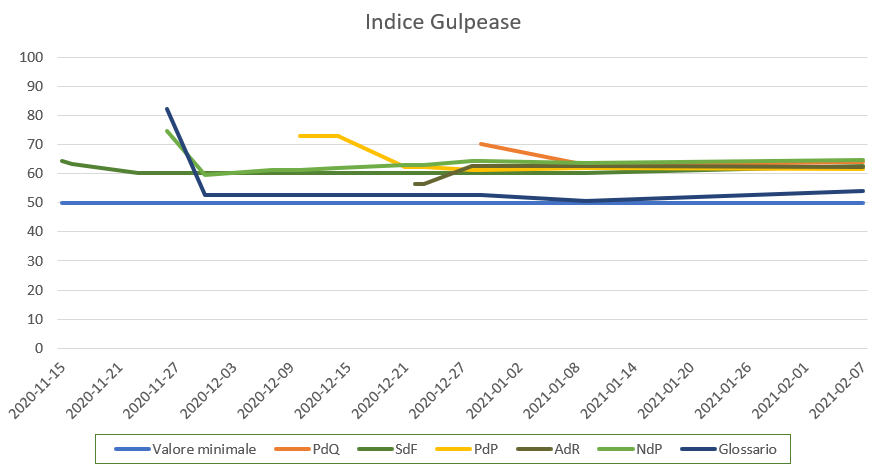
\includegraphics[scale=0.6]{Immagini/Gulpease_v1.1}
	\caption{Indice di Gulpease comprendente l'andamento di tutti i documenti}
	\label{fig:gulpease}
\end{figure}
\newpage
\subsubsection{Strategia adottata per l'analisi dinamica}
L'analisi dinamica di ciascun documento è stata eseguita mediante l'utilizzo dello strumento \glo{GitHub} Actions. Questo ha garantito una stesura del codice \LaTeX{} priva di errori semantici. Infatti, tramite questo strumento di verifica continua, è stato possibile individuare errori che potevano essere ignorati durante la compilazione locale del documento da qualche membro del team. Viene inviata una notifica ad ogni componente del gruppo sia in caso di successo che di fallimento portando il \textit{Verificatore} incaricato a dedicarsi alla risoluzione del problema in modo da avere sempre dei documenti compilabili e corretti.

\subsection{Periodo di progettazione architetturale}
Durante il periodo di progettazione architetturale, come nel periodo precedente, i documenti redatti da presentare in ingresso alla \textbf{Revisione di Progettazione} sono stati sottoposti a verifica secondo i criteri definiti nelle \NdPv{1.0.0}. In questo periodo sono stati valutati attraverso verifica anche i vari processi istanziati.
\subsubsection{Esiti verifica}
\myparagraph{SPICE}
A partire da questo periodo il gruppo ha applicato retrospettivamente lo standard SPICE per la cui descrizione si rimanda all'appendice delle \NdPv{2.0}. Di seguito vengono riportati in forma tabellare i risultati ottenuti per i principali processi istanziati durante il periodo. 
\begin{table} [H]
	\begin{center}
		\begin{tabular}{|C{3cm}|c|c|c|c|c|c|}
			\rowcolor{darkblue}
			\textcolor{white}{\textbf{Processo}}&
			\textcolor{white}{\textbf{Liv1}}&
			\textcolor{white}{\textbf{Liv2}}&
			\textcolor{white}{\textbf{Liv3}}&
			\textcolor{white}{\textbf{Liv4}}&
			\textcolor{white}{\textbf{Liv5}}&
			\textcolor{white}{\textbf{Risultato}} \\
				
			Fornitura & \textbf{PP:} & \textbf{PM:} \textbf{WMP:} & \textbf{PDEF:} \textbf{PDEP:} & \textbf{PC:} \textbf{PME:} &
			\textbf{PI:} \textbf{PO:} & \textbf{Inizio:} \textbf{Fine:} \\ \hline
			Documentazione & \textbf{PP:} & \textbf{PM:} \textbf{WMP:} & \textbf{PDEF:} \textbf{PDEP:} & \textbf{PC:} \textbf{PME:} &
			\textbf{PI:} \textbf{PO:} & \textbf{Inizio:} \textbf{Fine:} \\ \hline
			
			Sviluppo & \textbf{PP:} & \textbf{PM:} \textbf{WMP:} & \textbf{PDEF:} \textbf{PDEP:} & \textbf{PC:} \textbf{PME:} &
			\textbf{PI:} \textbf{PO:} & \textbf{Inizio:} \textbf{Fine:} \\ \hline
			
			Documentazione & \textbf{PP:} & \textbf{PM:} \textbf{WMP:} & \textbf{PDEF:} \textbf{PDEP:} & \textbf{PC:} \textbf{PME:} &
			\textbf{PI:} \textbf{PO:} & \textbf{Inizio:} \textbf{Fine:} \\ \hline
			
			Gestione della configurazione & \textbf{PP:} & \textbf{PM:} \textbf{WMP:} & \textbf{PDEF:} \textbf{PDEP:} & \textbf{PC:} \textbf{PME:} &
			\textbf{PI:} \textbf{PO:} & \textbf{Inizio:} \textbf{Fine:} \\ \hline
			
			Gestione della qualità & \textbf{PP:} & \textbf{PM:} \textbf{WMP:} & \textbf{PDEF:} \textbf{PDEP:} & \textbf{PC:} \textbf{PME:} &
			\textbf{PI:} \textbf{PO:} & \textbf{Inizio:} \textbf{Fine:} \\ \hline
			
			Verifica & \textbf{PP:} & \textbf{PM:} \textbf{WMP:} & \textbf{PDEF:} \textbf{PDEP:} & \textbf{PC:} \textbf{PME:} &
			\textbf{PI:} \textbf{PO:} & \textbf{Inizio:} \textbf{Fine:} \\ \hline	
		\end{tabular}
	\end{center}
\end{table}
\myparagraph{Documentazione}
\paragraph*{MPR02: Indice di Gulpease}
\paragraph*{MPR03: Indice di correttezza ortografica}
\myparagraph{Pianificazione}
\paragraph*{MPR04: Budget at Completion}
\paragraph*{MPR05: Actual Cost of Work Performed} \paragraph*{MPR06: Budget Cost of Work Performed} \paragraph*{MPR07: Budget Cost of Work Scheduled}
 \begin{figure}[ht]
	\centering
	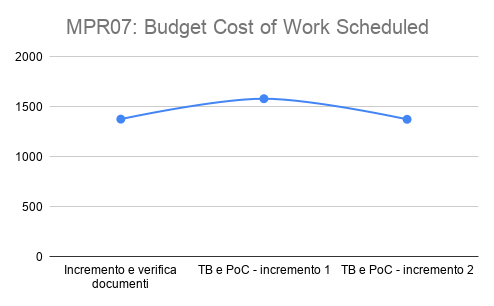
\includegraphics[scale=0.6]{Immagini/BCWS_PArchitetturale.png}
	\caption{BCWS progettazione architetturale}
	\label{fig:BCWS_PArchitetturale}
\end{figure}
 \paragraph*{MPR08: Schedule Variance}
\paragraph*{MPR09: Budget Variance}
\myparagraph{Miglioramento del processo}
\paragraph*{MPR10: Indice di risoluzione dei problemi}